\chapter{Machine Learning Models Explored}

This section describes the process of choosing the architectural and regularization hyperparamers for each model. The section also describes the datasets used to train the models 

The simplest model explored is the DNN. Because of the high dimension of the input data, feature extraction methods will be implemented and compared. These methods include PCA, a DAE, and a CAE. 

The other general architecture that will be explored is a 1D CNN. 

\subsection{Training Dataset Overview}

The datasets used to train the models are composed of noiseless simulated gamma-ray templates. A one-dimension particle transport code developed at Sandia National Laboratory, GADRAS-DRF, was used to generate these templates. This simulation code can be used to model the conditions that effect spectra. The parameters used in this study are different detector materials, detector size, environmental scattering factors, shielding, and background as a function of location. GADRAS-DRF includes an option to create spectra without the Poisson noise expected for a spectrum. Using this, noiseless templates were generated.

The parameters simulated are based on handheld RIID scenarios. The source-detector height from ground are sampled between values shin and arm height. 


\begin{table}[H]
\centering
\begin{tabular}{|c|c|}
\hline
Parameter & Values \\ \hline
\begin{tabular}[c]{@{}c@{}}source-detector height \\ off ground {[}cm{]}\end{tabular} & 50.0, 75.0, 100.0, 125.0, 150.0 \\ \hline
\begin{tabular}[c]{@{}c@{}}source-detector\\ distance {[}cm{]}\end{tabular} & \multicolumn{1}{l|}{50.0, 112.5, 175.0, 237.5, 300.0} \\ \hline
\begin{tabular}[c]{@{}c@{}}Arial density of \\ solid aluminum {[}g/cm\textasciicircum{}2{]}\end{tabular} & 1.82, 4.18, 7.49, 13.16 \\ \hline
\begin{tabular}[c]{@{}c@{}}Arial density of\\  solid iron {[}g/cm\textasciicircum{}2{]}\end{tabular} & 1.53, 3.5, 6.28, 11.02 \\ \hline
\begin{tabular}[c]{@{}c@{}}Arial density of \\ solid lead {[}g/cm\textasciicircum{}2{]}\end{tabular} & 0.22, 0.51, 0.92, 1.61 \\ \hline
\begin{tabular}[c]{@{}c@{}}FWHM at\\  662 keV {[}\%{]}\end{tabular} & \multicolumn{1}{l|}{6.0, 6.5, 7.0, 7.5, 8.0, 8.5, 9.0} \\ \hline
\end{tabular}
\caption{Fixed GADRAS-DRF simulation parameters.}
\label{table:all_fixed_simulation_parameters}
\end{table}

\begin{table}[H]
\centering
\begin{tabular}{|c|c|c|}
\hline
Parameter & Values & Sampling \\ \hline
integration time & 60 - 600 & uniform \\ \hline
background counts per second & 200 & Poisson \\ \hline
Signal to Background ratio & 0.5 - 2 & uniform \\ \hline
0th order calibration & 0 - 10 & uniform \\ \hline
1st order calibration & 0.83 - 1.16 & uniform \\ \hline
2nd order calibration & 0 - 0 & uniform \\ \hline
\end{tabular}
\caption{Default data augmentation parameters.}
\label{table:all_variable_simulation_parameters}
\end{table}

Spectra change due to changes in measurement geometry. These changes include source-to-detector distance and the distance of both the detector and source from objects in an environment. To demonstrate this effect, $^{60}$Co spectra were simulated, Figure \ref{fig:sim_spectra_distance_comparison}, with different source-to-detector distances.

$^{60}$Co spectra were also simulated at different distances from the ground, shown in Figure \ref{fig:sim_spectra_height_comparison}.



\begin{figure}[H]
\centering
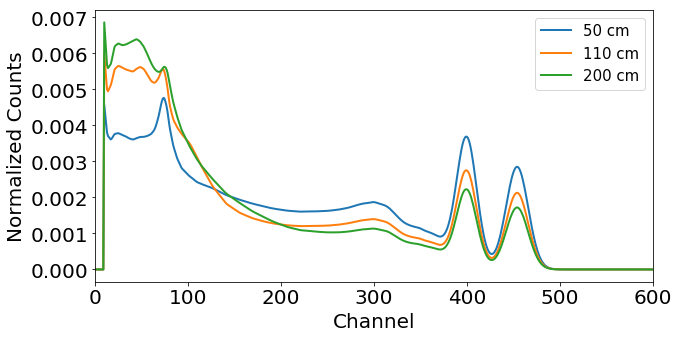
\includegraphics[width=0.95\linewidth]{images/sim_spectra_distance_comparison}
\caption{Comparison of a $^{60}$Co spectrum simulated at various source-detector distances.}
\label{fig:sim_spectra_distance_comparison}
\end{figure}

\begin{figure}[H]
\centering
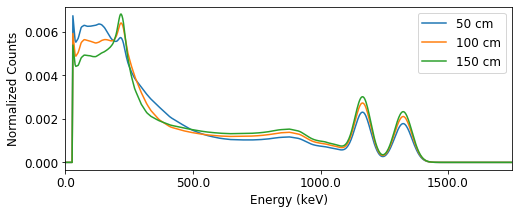
\includegraphics[width=0.95\linewidth]{images/sim_spectra_height_comparison}
\caption{Comparison of a $^{60}$Co spectrum simulated at various source-detector heights off the ground.}
\label{fig:sim_spectra_height_comparison}
\end{figure}



To incorporate these changes, templates simulated at different distances are included in the dataset. These distances start at 30cm, which is the distance at which a 1 uCi source will have an activity of about 400 cps on a 2 inch diameter detector. This is about twice the expected activity of background. 

Changes in calibration due to temperature shifts are also considered. Due to the relatively large magnitude in calibration shifts due to temperature shifts from -5 C to 40 C \cite{CASANOVAS2012588}, it is expected incorporating these additions will also make the algorithm robust against calibration.

Different NaI(Tl) detectors have different amounts of peak Gaussian broadening. Spectra are also simulated with different FWHM parameters.


\begin{figure}[H]
\centering
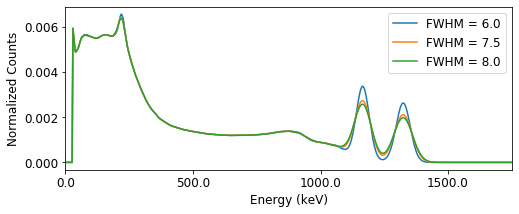
\includegraphics[width=0.95\linewidth]{images/sim_spectra_FWHM_comparison}
\caption{Comparison of a $^{60}$Co spectrum simulated with various FWHM parameters.}
\label{fig:sim_spectra_FWHM_comparison}
\end{figure}


\section{Datasets Used for the Hyperparameter Search}

To show generalization improvements from including more physical parameters in the simulated dataset, networks will be trained on two datasets. Because datasets of different complexity often need different architectures and hyperparameters \cite{Bergstra2012}, independent hyperparameter searches will be conducted for each dataset. The first dataset is comprised of unshielded gamma-ray spectra of ANSI isotopes simulated using GADRAS. Each spectrum has parameters randomly selected from Table \ref{table:hyperparameter_dataset_easy_parameters}. The average training error from 5-fold cross validation training using early stopping patience of 20 epochs was used to train 128 models. The maximum number of epochs was set to 200. A total of 1000 spectra are simulated for each isotope for the DNN. A total of 100 spectra are simulated for each isotope for the CNN due to computational constraints training the CNN.

\begin{table}[H]
\centering
\caption{Range of parameters used for the simple dataset.}
\label{table:hyperparameter_dataset_easy_parameters}
\begin{tabular}{c|c|c|}
\cline{2-3}
 & Hyperparameter Range & Sampling \\ \hline
\multicolumn{1}{|c|}{Source-Detector Distance {[}cm{]}} & 175.0 & N/A \\ \hline
\multicolumn{1}{|c|}{Source-Detector Height {[}cm{]}} & 100.0 & N/A \\ \hline
\multicolumn{1}{|c|}{FWHM 662 keV {[}s{]}} & 7.5 & N/A \\ \hline
\multicolumn{1}{|c|}{\begin{tabular}[c]{@{}c@{}}Shielding\\ (Percent 662 keV Attenuated)\end{tabular}} & 0\%, 20\% & Uniform \\ \hline
\multicolumn{1}{|c|}{Integration Time {[}s{]}} & 60 - 3600 & Uniform \\ \hline
\multicolumn{1}{|c|}{Linear Calibration Offset} & 0.8 - 1.2 & Uniform \\ \hline
\multicolumn{1}{|c|}{Signal to Background Ratio} & 0.5 - 2.0 & Uniform \\ \hline
\end{tabular}
\end{table}


\begin{table}[H]
\centering
\caption{Range of parameters used for the full dataset.}
\label{table:hyperparameter_dataset_full_parameters}
\begin{tabular}{c|c|c|}
\cline{2-3}
 & Hyperparameter Range & Sampling \\ \hline
\multicolumn{1}{|c|}{Source-Detector Distance {[}cm{]}} & 50.5, 175.0, 300 & Uniform \\ \hline
\multicolumn{1}{|c|}{Source-Detector Height {[}cm{]}} & 50, 100.0, 150 & Uniform \\ \hline
\multicolumn{1}{|c|}{FWHM 662 keV {[}s{]}} & 7.0, 7.5, 8.0 & Uniform \\ \hline
\multicolumn{1}{|c|}{\begin{tabular}[c]{@{}c@{}}Shielding\\ (Percent 662 keV Attenuated)\end{tabular}} & 0\%, 20\%, 40\%, 60\% & Uniform \\ \hline
\multicolumn{1}{|c|}{Integration Time {[}s{]}} & 60 - 3600 & Uniform \\ \hline
\multicolumn{1}{|c|}{Linear Calibration Offset} & 0.8 - 1.2 & Uniform \\ \hline
\multicolumn{1}{|c|}{Signal to Background Ratio} & 0.5 - 2.0 & Uniform \\ \hline
\end{tabular}
\end{table}


\section{Hyperparameter Search Results}

The results of the hyperparameter searches are shown using random efficiency curves and by comparing parameter values versus F1 score in the training set.

Random efficiency curves indicate the quality of the hyperparameter search space and allow for reproducibility. 


% These also allow for researchers who want to fit models to this dataset to have a performance benchmark. If you wanted to compare random hyperparameter search to more intelligent methods, you could compare using this.

\subsection{Dense Architecture}

Architecture and training hyperparamters are shown in Table \ref{table:hyperparameter_dataset_parameters_DNN}. Note, the number of nodes in each layers was made to decrease for each subsequent layer.

\begin{table}[H]
\centering
\caption{Range of hyperparameter explored for the DNN.}
\label{table:hyperparameter_dataset_parameters_DNN}
\begin{tabular}{c|c|c|}
\cline{2-3}
 & Hyperparameter Range & Sampling \\ \hline
\multicolumn{1}{|c|}{Number of Layers} & 1 - 3 & Uniform \\ \hline
\multicolumn{1}{|c|}{Nodes in Layer} & 2$^{5}$ - 2$^{10}$ & Power of Two \\ \hline
\multicolumn{1}{|c|}{Initial Learning Rate} & 10$^{-4}$ - 10$^{-1}$ & Logarithmic \\ \hline
\multicolumn{1}{|c|}{L2 Regularization Strength} & 10$^{-2}$ - 10$^{0}$ & Logarithmic \\ \hline
\multicolumn{1}{|c|}{Dropout Frequency} & 0 - 1 & Uniform \\ \hline
\multicolumn{1}{|c|}{Batch Size} & 2$^{4}$ - 2$^{10}$ & Power of Two \\ \hline
\multicolumn{1}{|c|}{Activation Function} & relu, tanh & Uniform \\ \hline
\multicolumn{1}{|c|}{Input Scaling} & sqrt, log1p & Uniform \\ \hline
\end{tabular}
\end{table}



Random efficiency curves for different reprocessing methods for the DNN are shown in Figure \ref{fig:random_hp_search_dnn_easy}. This figure implies that the optimum prepossessing step is BLANK. It's interesting that BLANK does better than BLANK.

\begin{figure}[H]
	\centering
	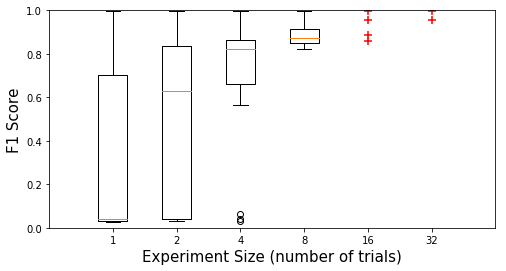
\includegraphics[width=0.8\linewidth]{images/random_hp_search_dnn_easy}
	\caption{Random hyperparameter search efficiency curves for the DNN using the first dataset.}
	\label{fig:random_hp_search_dnn_easy}
\end{figure}

\begin{figure}[H]
	\centering
	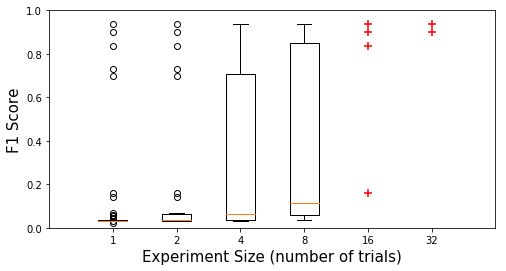
\includegraphics[width=0.8\linewidth]{images/random_hp_search_dnn_full}
	\caption{Random hyperparameter search efficiency curves for the DNN using the second dataset.}
	\label{fig:random_hp_search_dnn_full}
\end{figure}


Figure \ref{fig:dense_hyperparameters_f1_score} shows the distribution of random hyperparameters and their average F1 score from the k-folds testing set. Sub-figure \ref{fig:learning_rate_learning} shows that a learning rate less than 10$^{-2}$ should be used for future hyperparameter searches. This figure also shows that the more difficult dataset prefers a slower learning rate. 


\begin{figure}[H]
     \centering
     \begin{subfigure}[b]{0.49\textwidth}
         \centering
         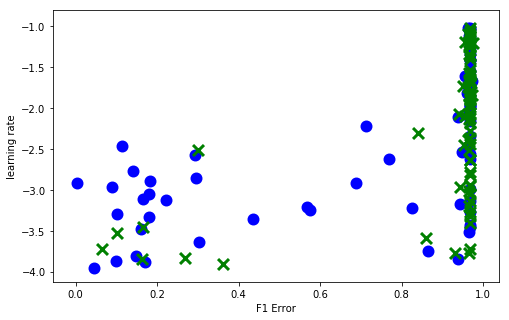
\includegraphics[width=\textwidth]{images/learning_rate_dummy.png}
         \caption{Learning Rate}
         \label{fig:learning_rate_learning}
     \end{subfigure}
     \hfill
     \begin{subfigure}[b]{0.49\textwidth}
         \centering
         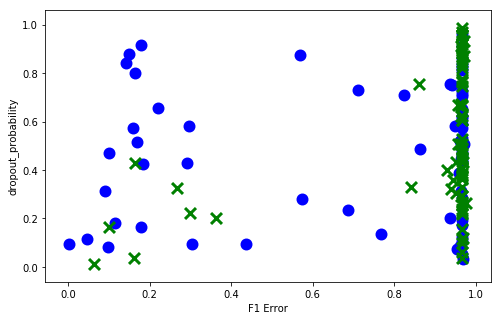
\includegraphics[width=\textwidth]{images/dropout_dummy.png}
         \caption{Dropout Rate}
         \label{fig:dropout_learning}
     \end{subfigure}

     \begin{subfigure}[b]{0.49\textwidth}
         \centering
         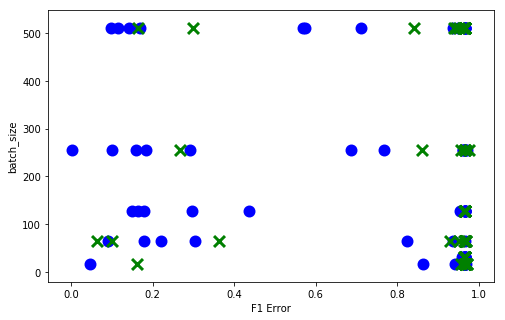
\includegraphics[width=\textwidth]{images/batch_size_dummy.png}
         \caption{Batch Size}
         \label{fig:batch_size_learning}
     \end{subfigure}
     \hfill
     \begin{subfigure}[b]{0.49\textwidth}
         \centering
         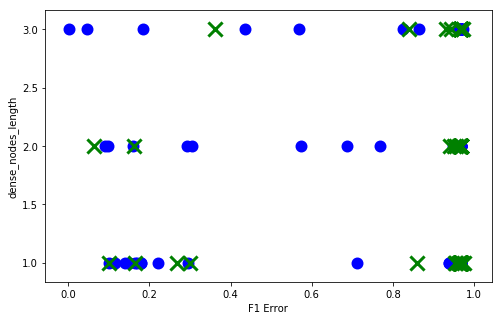
\includegraphics[width=\textwidth]{images/dense_layers_total_dummy.png}
         \caption{Total Dense Layers}
         \label{fig:dense_layers_learning}
     \end{subfigure}

    \begin{subfigure}[b]{0.49\textwidth}
         \centering
         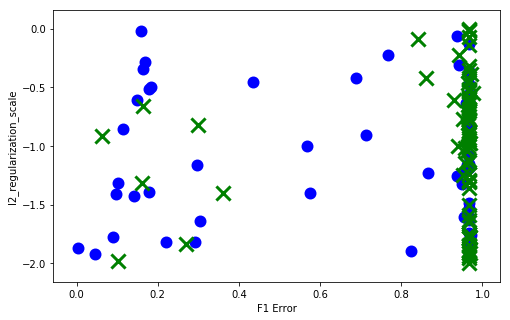
\includegraphics[width=\textwidth]{images/l2_reg_dummy.png}
         \caption{L2 Regularization Scale}
         \label{fig:L2_scale_learning}
     \end{subfigure}
     \hfill
     \begin{subfigure}[b]{0.49\textwidth}
         \centering
         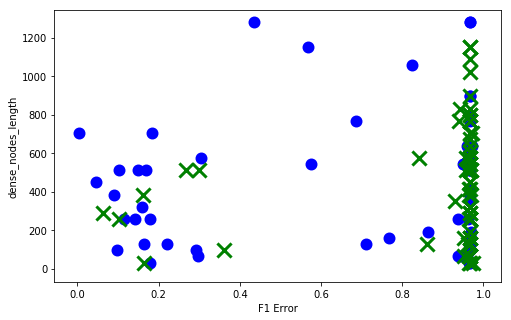
\includegraphics[width=\textwidth]{images/dense_nodes_total_dummy.png}
         \caption{Total Nodes}
         \label{fig:total_nodes_learning}
     \end{subfigure}     
        \caption{Effect of hyperparameters on F1 score. Blue circles represent the simple dataset, green crosses are the complete dataset.}
        \label{fig:dense_hyperparameters_f1_score}
\end{figure}


In addition to hyperparameters associated with the DNN's architecture and training, hyperparameters explored include the autoencoder used. Autoencoders can generate a different encoding based on a given architecture. The mean squared reconstruction error may not be the best metric to measure how good this encoding is as a preprocessing step. To determine an optimum preprocessing architecture for the dense and convolutional autoencoder, the choice of preprocessing architectures was added as a hyperparameter. The choices belong to the set with the N best reconstruction errors, respective of dense and convolution architecture.

% \subsubsection{Hyperparameter Search Results - Autoencoders}

% Now that we know optimized autoencoder architectures for the DNN, we need to optimize training hyperparameters. 

% https://machinelearningmastery.com/activation-regularization-for-reducing-generalization-error-in-deep-learning-neural-networks/

% \cite{Ranzato2007} Fig 6 shows you can freeze the unsupervised feature extraction network and update the classifier if you have enough data.

% Sparse denoising autoencoders are included in in this work as feature extraction and dimension reduction techniques. Both autoencoders employ regularization techniques to ensure useful representations are learned. Both models includes $l1$ activity regularization as a method to induce sparsity on the networks activations, which increases generalization \cite{Goodfellow-et-al-2016}. 

% Show how well autoencoders worked at spectrum reconstruction and background subtraction. See if there's a large difference between doing background subtraction and 


\subsection{Convolution Architecture}

Just like the autoencoder, this can be done in one or two steps. One step: Train and optimize the entire network, convolution and dense layers. Two steps: Train and optimize the dense layer, using random initialization for non-trainable convolution filters. We'll probably go with the two-step.

\begin{table}[H]
\centering
\caption{Range of hyperparameter explored for the CNN.}
\label{table:hyperparameter_dataset_parameters_CNN}
\begin{tabular}{c|c|c|}
\cline{2-3}
 & Hyperparameter Range & Sampling \\ \hline
\multicolumn{1}{|c|}{Number of Filter Kernels} & \begin{tabular}[c]{@{}c@{}}(4)   (8)   (16)    (32)\\ (4, 8)  (8, 16)  (16, 32)\\ (4, 8, 16)   (8, 16, 32)\end{tabular} & Uniform \\ \hline
\multicolumn{1}{|c|}{Filter Kernel Length} & 2, 4, 8, 16 & Uniform \\ \hline
\multicolumn{1}{|c|}{Pooling size} & 2, 4, 8, 16 & Uniform \\ \hline
\multicolumn{1}{|c|}{Number of Dense Layers} & 1 - 3 & Uniform \\ \hline
\multicolumn{1}{|c|}{Nodes in Dense Layers} & 10 - 1000 & Logarithmic \\ \hline
\multicolumn{1}{|c|}{Initial Learning Rate} & 10$^{-4}$ - 10$^{-1}$ & Logarithmic \\ \hline
\multicolumn{1}{|c|}{L2 Regularization Strength} & 10$^{-2}$ - 10$^{0}$ & Logarithmic \\ \hline
\multicolumn{1}{|c|}{Dropout Frequency} & 0 - 1 & Uniform \\ \hline
\multicolumn{1}{|c|}{Batch Size} & 2$^{4}$ - 2$^{6}$ & Power of Two \\ \hline
\multicolumn{1}{|c|}{Activation Function} & tanh & Uniform \\ \hline
\multicolumn{1}{|c|}{Input Scaling} & sqrt, log1p & Uniform \\ \hline
\end{tabular}
\end{table}


\begin{figure}[H]
	\centering
	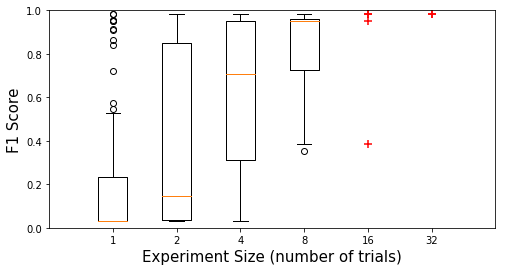
\includegraphics[width=0.8\linewidth]{images/random_hp_search_cnn_easy}
	\caption{Random hyperparameter search efficiency curves for the CNN using the first dataset.}
	\label{fig:random_hp_search_cnn_easy}
\end{figure}

\begin{figure}[H]
	\centering
	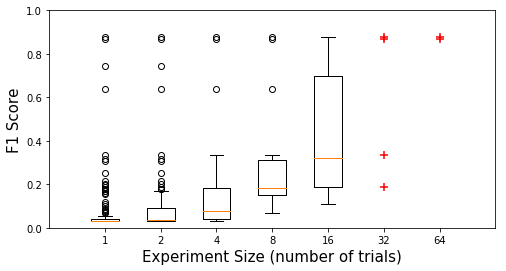
\includegraphics[width=0.8\linewidth]{images/random_hp_search_cnn_full}
	\caption{Random hyperparameter search efficiency curves for the CNN using the second dataset.}
	\label{fig:random_hp_search_cnn_full}
\end{figure}





Figure \ref{fig:cnn_hyperparameters_f1_score} shows the distribution of random hyperparameters from the CNN and their average F1 score from the k-folds testing set. 


\begin{figure}[H]
     \centering
     \begin{subfigure}[b]{0.49\textwidth}
         \centering
         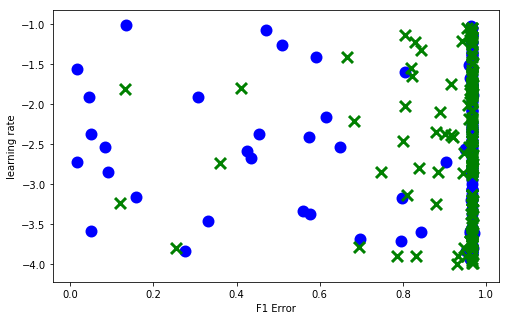
\includegraphics[width=\textwidth]{images/cnn_learning_rate_dummy.png}
         \caption{Learning Rate}
         \label{fig:cnn_learning_rate_learning}
     \end{subfigure}
     \hfill
     \begin{subfigure}[b]{0.49\textwidth}
         \centering
         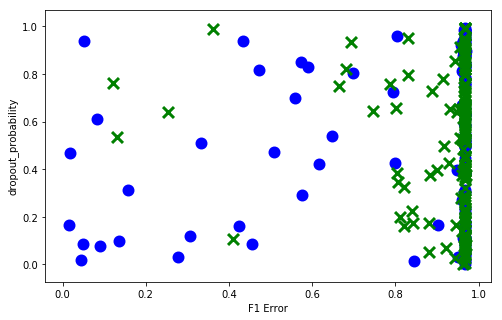
\includegraphics[width=\textwidth]{images/cnn_dropout_dummy.png}
         \caption{Dropout Rate}
         \label{fig:cnn_dropout_learning}
     \end{subfigure}

     \begin{subfigure}[b]{0.49\textwidth}
         \centering
         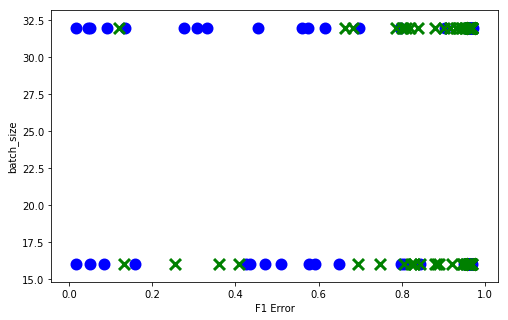
\includegraphics[width=\textwidth]{images/cnn_batch_size_dummy.png}
         \caption{Batch Size}
         \label{fig:cnn_batch_size_learning}
     \end{subfigure}
     \hfill
     \begin{subfigure}[b]{0.49\textwidth}
         \centering
         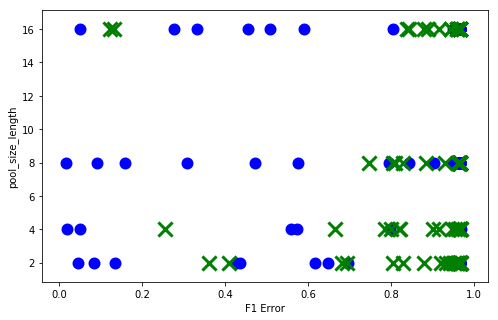
\includegraphics[width=\textwidth]{images/cnn_pooling_size_dummy.png}
         \caption{CNN Pooling Size}
         \label{fig:cnn_dense_layers_learning}
     \end{subfigure}

    \begin{subfigure}[b]{0.49\textwidth}
         \centering
         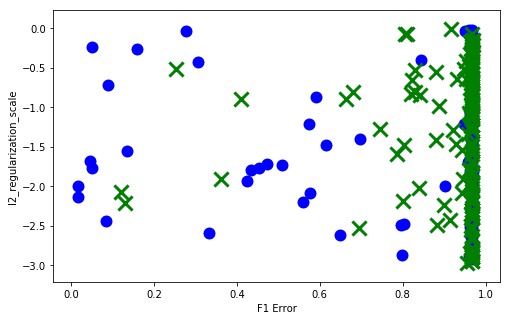
\includegraphics[width=\textwidth]{images/cnn_l2_reg_dummy.png}
         \caption{L2 Regularization Scale}
         \label{fig:cnn_L2_scale_learning}
     \end{subfigure}
     \hfill
     \begin{subfigure}[b]{0.49\textwidth}
         \centering
         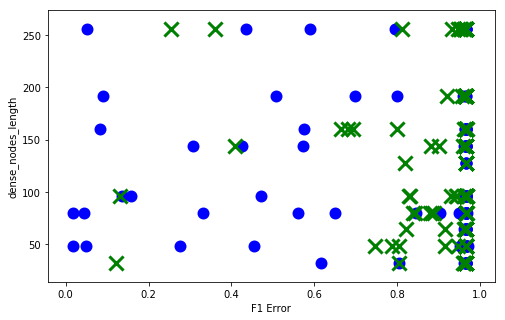
\includegraphics[width=\textwidth]{images/cnn_dense_nodes_total_dummy.png}
         \caption{Total Dense Nodes}
         \label{fig:cnn_total_nodes_learning}
     \end{subfigure}  
     
     \begin{subfigure}[b]{0.49\textwidth}
         \centering
         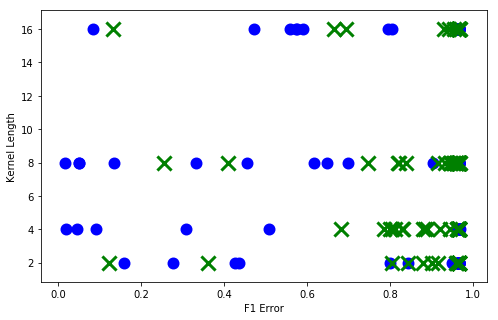
\includegraphics[width=\textwidth]{images/cnn_kernel_length_dummy.png}
         \caption{Convolution Kernel Length}
         \label{fig:cnn_L2_scale_learning}
     \end{subfigure}
     \hfill
     \begin{subfigure}[b]{0.49\textwidth}
         \centering
         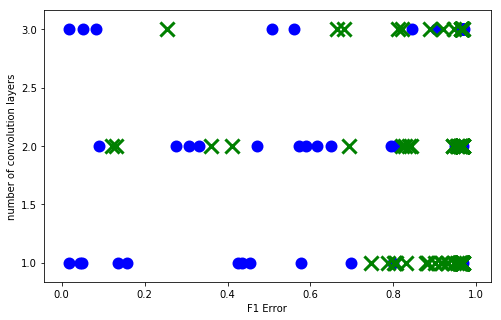
\includegraphics[width=\textwidth]{images/cnn_num_conv_layers_dummy.png}
         \caption{Total Convolution Layers}
         \label{fig:cnn_total_nodes_learning}
     \end{subfigure}  
     
        \caption{Effect of CNN hyperparameters on F1 score. Blue circles represent the simple dataset, green crosses are the complete dataset.}
        \label{fig:cnn_hyperparameters_f1_score}
\end{figure}


\section{Autoencoder Architectures}

Without an autoencoder, a single ANN has to learn multiple tasks to identify isotopes. An ANN would have to simultaneously identify the detector calibration, background signal, and source signal. By training an autoencoder to reconstruct a background-subtracted and correctly calibrated spectrum, the task of isotope identification is simplified for the ANN. This may result in more accurate identifications. 




To test this, for each dataset a single autoencoder and three ANNs will be trained. The first will be trained without an autoencoder. The second will be trained using the encoder as input. A random hyperparameter search will be used to find an appropriately structured autoencoder. The testing and validation error for these ANNs will be compared for each respective dataset.

\subsection{Autoencoder Structure Hyperparameter Search}

This section will explain the hyperparameter structures searched. The autoencoder used is a undercomplete denoising autoencoder \cite{Goodfellow-et-al-2016}. Because the denoising operation performs regularization, no additional regularization is added to these models.


Figure \ref{fig:autoencoder_real_spectra} shows the autoencoder performance on real spectra, showing good performance.

\begin{figure}[H]
	\centering
	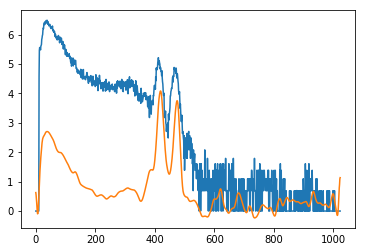
\includegraphics[width=0.8\linewidth]{images/bscae_example.png}
	\caption{Example autoencoder decoding performance on real spectra.}
	\label{fig:autoencoder_real_spectra}
\end{figure}


\subsection{Autoencoder Performance - As Pretraining or as Feature Extractor}

This section will compare how well the autoencoders perform as pretrained networks and as feature extractors for a DNN. To do this, a trained CAE and DAE will be connected to a dense network. These will be trained to either fixing the autoencoder's weights or by fine-tuning them while the network learns.


\begin{table}[H]
\centering
\caption{Range of hyperparameter explored for the DAE.}
\label{table:hyperparameter_dataset_parameters_DAE}
\begin{tabular}{c|c|c|}
\cline{2-3}
 & Hyperparameter Range & Sampling \\ \hline
\multicolumn{1}{|c|}{Number of Layers} & 1 - 3 & Uniform \\ \hline
\multicolumn{1}{|c|}{Nodes in Layer} & 2$^{5}$ - 2$^{10}$ & Power of Two \\ \hline
\multicolumn{1}{|c|}{Initial Learning Rate} & 10$^{-4}$ - 10$^{-1}$ & Logarithmic \\ \hline
\multicolumn{1}{|c|}{L2 Regularization Strength} & 10$^{-2}$ - 10$^{0}$ & Logarithmic \\ \hline
\multicolumn{1}{|c|}{Dropout Frequency} & 0 - 1 & Uniform \\ \hline
\multicolumn{1}{|c|}{Batch Size} & 2$^{4}$ - 2$^{10}$ & Power of Two \\ \hline
\multicolumn{1}{|c|}{Activation Function} & relu, tanh & Uniform \\ \hline
\multicolumn{1}{|c|}{Input Scaling} & sqrt, log1p & Uniform \\ \hline
\end{tabular}
\end{table}











\begin{table}[H]
\centering
\caption{Comparison of fixed and pretrained autoencoders.}
\label{table:autoencoders_fixed_pretrained}
\begin{tabular}{|c|c|}
\hline
Model & Test Set F1 Score \\ \hline
\begin{tabular}[c]{@{}c@{}}CAE-DNN\\ fixed\end{tabular} & 0.4 \\ \hline
\begin{tabular}[c]{@{}c@{}}CAE-DNN as\\ pretraining\end{tabular} & 0.4 \\ \hline
\begin{tabular}[c]{@{}c@{}}DAE-DNN\\ fixed\end{tabular} & 0.4 \\ \hline
\begin{tabular}[c]{@{}c@{}}DAE-DNN as\\ pretraining\end{tabular} & 0.4 \\ \hline
\end{tabular}
\end{table}




\begin{figure}[H]
	\centering
	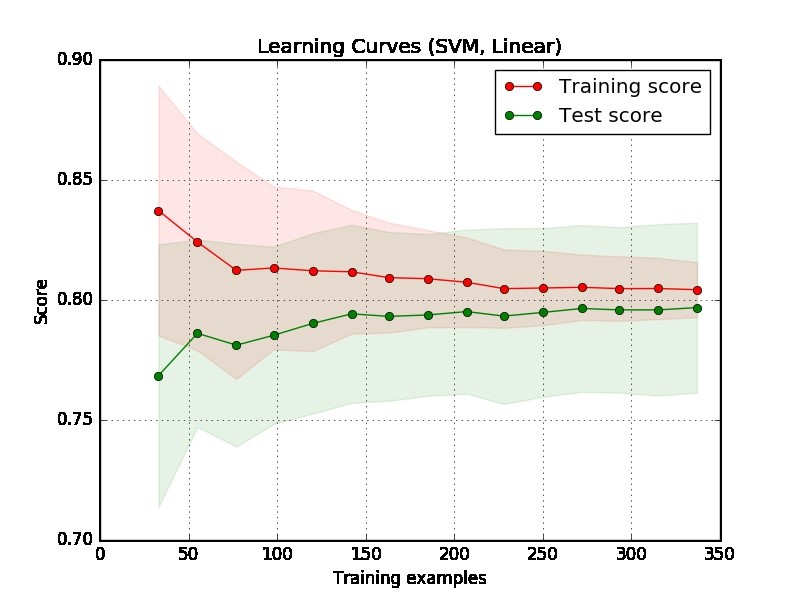
\includegraphics[width=0.8\linewidth]{model_choice_hyperparameter_search_images/learning_curve_dummy}
	\caption{Training curves for the fixed and pretraining DAE-DNN's, CAE-DNN's.}
	\label{fig:learning_curves}
\end{figure}




\section{Summary of Final Model Architectures}


This section discusses performance differences between the DNN, CNN, CAE-DNN, and DAE-DNN. These differences will be based on the final testing set error for all models.  





